\documentclass[main.tex]{subfiles}

\begin{document}

	\begingroup

	\renewcommand{\cleardoublepage}{}

	\renewcommand{\clearpage}{}

	\chapter{Navigation Function Documentation}

		\chapterauthor{Marc Stelter}
		
		\section{mapping\_hector\_slam}
		It contains a simple launch file starting hector\_slam with the correct parameters for the HSR.
		
		\section{obstacle\_finder.py}\label{met_obstacle_finder}
		Uses the laser scanner in accordance with the map to find objects.
		
		\begin{itemize}
			\item Input: 
				\subitem nav\_msgs/OccupancyGrid
				\subitem sensor\_msgs/LaserScan
			\item Parameter:
				\subitem occ\_threshold 
				Minimum value for a cell in the OccupancyGrid to be occupied
				\subitem min\_scans\_cluster
				Minimum number of laser rays to form a cluster
				\subitem min\_percentage\_covered
				Percentage of a cluster covered by the map to be part of it
				\subitem rad\_neighbor (m)
				Max distance between cells of a cluster
				\subitem error\_map (m)
				Allowed deviation in the map
				\subitem use\_every\_n\_scan
				Skip ecery nth LaserScan message 
			\item  Publish:
				\subitem Topic: /object\_finder
				\subitem Type: geometry\_msgsPoseArray
		\end{itemize}
	
		\subsection{How it works}
		
		\subsubsection{Intro}
		
		To better understand how the obstacle finder works it is important to understand how the world is represented in the map. In this case a \href{http://docs.ros.org/kinetic/api/nav_msgs/html/msg/OccupancyGrid.html}{Occupancy Grid} is used.
		
		\begin{figure}[H]
			\centering
			\includegraphics[width=0.7\textwidth]{pictures/obstacle_finder/Gridmap.pdf}
			\caption{Ros Occupancy Grid}
			\label{img_occ_grid}
		\end{figure}
		
		The figure \ref{img_occ_grid} visualizes an Occupancy Grid. For each position in the real world the corresponding x, y index gets calculated based on the resolution. Meaning each cell represents a certain are in the real world. In order to represent negative positions the world position (0,0) is explicitly represented. The values in each cell determine the probability of this cell being occupied. Ranging from 0 (free) to 255 (occupied).
		
		Next it is important to also understand the \href{http://docs.ros.org/melodic/api/sensor_msgs/html/msg/LaserScan.html}{Laser Scan}. 
		\begin{figure}[H]
			\centering
			\includegraphics[width=0.7\textwidth]{pictures/obstacle_finder/laserSnan.pdf}
			\caption{Ros Laser Scan}
			\label{img_laser_scan}
		\end{figure}
		 
		Figure \ref{img_laser_scan} represents the  aspects of the laser scan that are used by the obstacle finder. The scan consists of multiple rays each with their range in m. The min angle is the start angle of the scan. The angle increments represents the angular distance between each scan and the max angle the end angle of the scan.
		
		\subsubsection{Detecting an obstacle}
		
		\begin{figure}[H]
			\centering
			\includegraphics[width=0.7\textwidth]{pictures/obstacle_finder/Cluster-building.pdf}
			\caption{Finding clusters}
			\label{img_finding_cluster}
		\end{figure}   
	
		Figure \ref{img_finding_cluster} is a representation of the occupancy grid with the HSR in it and some exemplary rays of the scanner. In order to find obstacles the rays of a scan get bundled into a cluster. A cluster is a simple Array of the indexes of a ray in the occupancy grid.
		The first step to build clusters from these rays is to determine where the ray ends in the map. This is done by first getting the position of the laser scanner in the map by looking up its transform.
		
		Calculation of the position in the map:\\		
		$range = range of the ray$\\
		$angle = min\_angle + (ray\_index * angle\_increment)$
		
		$x = range * math.cos(angle + hsr.theta) + hsr.x$\\
		$y = range * math.sin(angle + hsr.theta) + hsr.y$\\
		
		Calculation of the indexes in the occupancy grid:\\
		$ix = int((x - origin.x) / resolution)$\\
		$iy = int((y - origin.y) / resolution)$
		
		For the following cluster building only the indexes are considered.
		
		\begin{figure}[H]
			\centering
			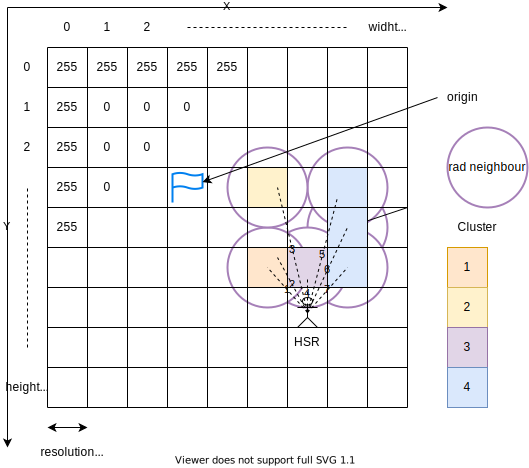
\includegraphics[width=0.7\textwidth]{pictures/obstacle_finder/Cluster-building2.pdf}
			\caption{Finding clusters}
			\label{img_building_cluster}
		\end{figure}
		
		\section{nav\_fix.py}
		A small node that takes in the original navigation goal and publishes an intermediate goal upon failure. The original goal gets published 3 times.
		
		This small node has proven to be useful inside the HSR lab since some cables seem to be triggering the magnetic sensors.

	\endgroup

\end{document}

